%================================================================
\section{Results and Discussion}\label{sec:Results}
%================================================================

%----------------------------------------------------------------
\subsection{Verifying the Implementation}\label{sec:project results}
%----------------------------------------------------------------

%----------------------------------------------------------------
\subsubsection{Non-Interacting}
%----------------------------------------------------------------

\autoref{fig:gridsearch} shows a VMC computations for a grid of $\alpha$ values for the non-interacting system for both the analytical and automatic differentiation approaches. 

\begin{figure}[H]
\centering
\subfloat[]{{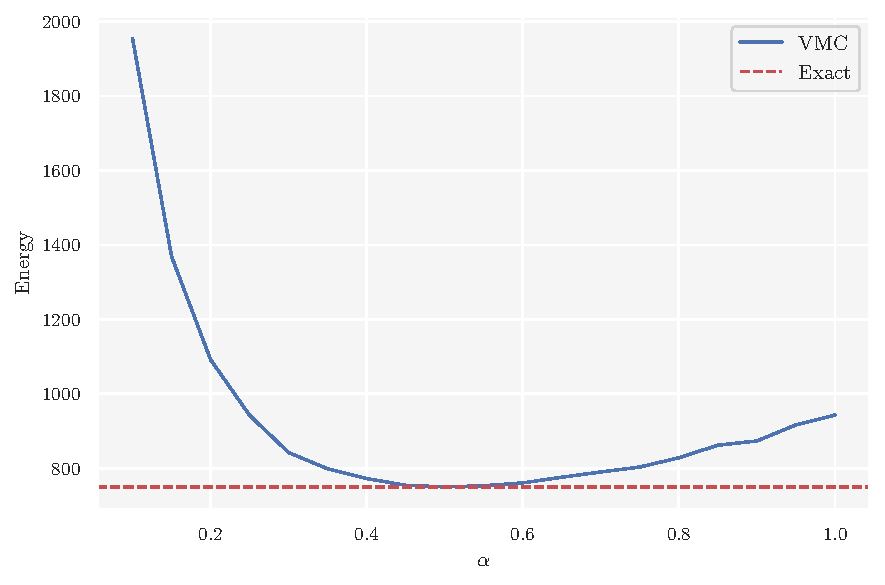
\includegraphics[scale=0.5]{latex/figures/grid_search_analytical.pdf}}}
\qquad
\subfloat[]{{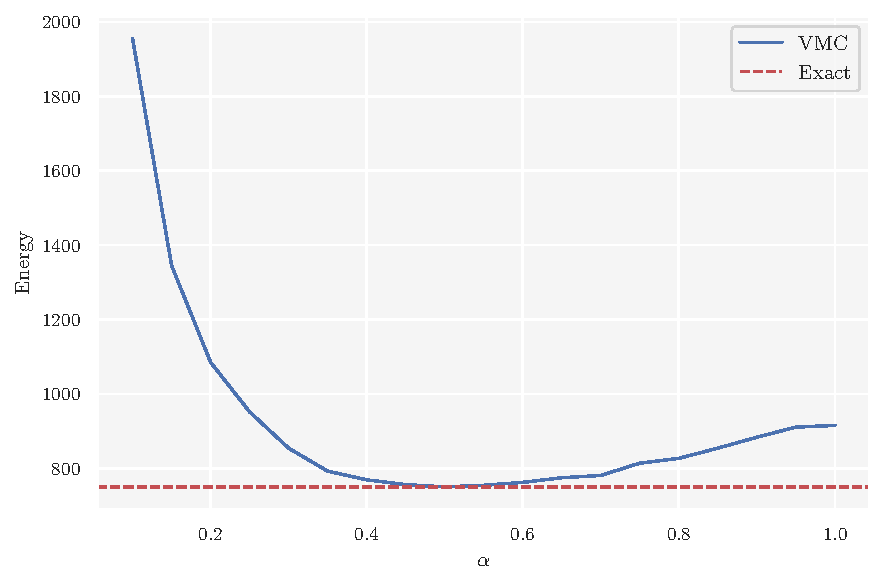
\includegraphics[scale=0.5]{latex/figures/grid_search_numerical.pdf}}}
\caption{Grid search $\alpha$, non-interacting system. \textbf{(a)} VMC computations with analytical expressions. \textbf{(b)} VMC computations with automatic differentiation.}
\label{fig:gridsearch}
\end{figure}



Discussion

%----------------------------------------------------------------
\subsubsection{Interacting}
%----------------------------------------------------------------

Compare log vs normal

%----------------------------------------------------------------
\subsection{Variational Energy}
%----------------------------------------------------------------

%----------------------------------------------------------------
\subsubsection{Non-Interacting}
%----------------------------------------------------------------

Discussion

\autoref{fig:non-interact_boxplot} shows 

\begin{figure}[!htb]
\centering
\subfloat[]{{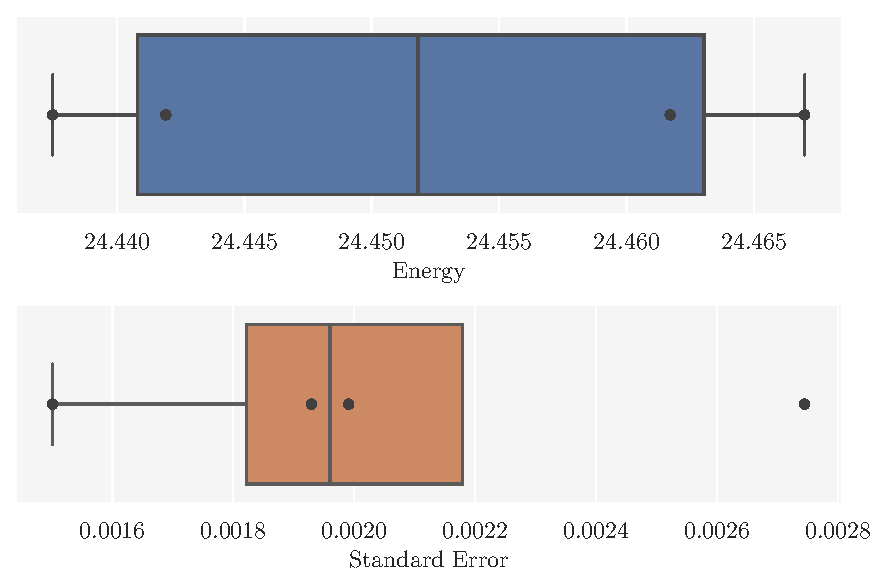
\includegraphics[scale=0.5]{latex/figures/boxplot_analytical_metropolis.pdf}}}
\qquad
\subfloat[]{{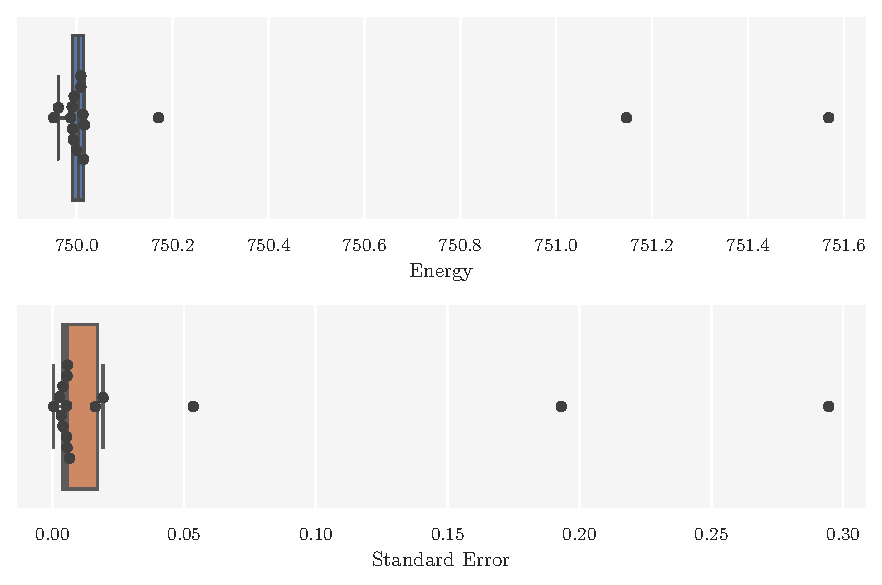
\includegraphics[scale=0.5]{latex/figures/boxplot_analytical_metropolis_hastings.pdf}}}
\qquad
\subfloat[]{{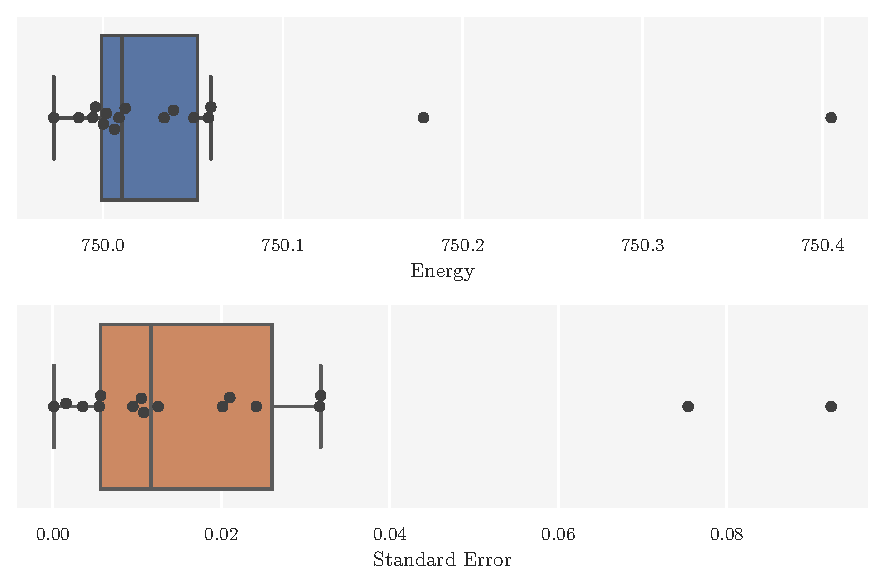
\includegraphics[scale=0.5]{latex/figures/boxplot_numerical_metropolis.pdf}}}
\qquad
\subfloat[]{{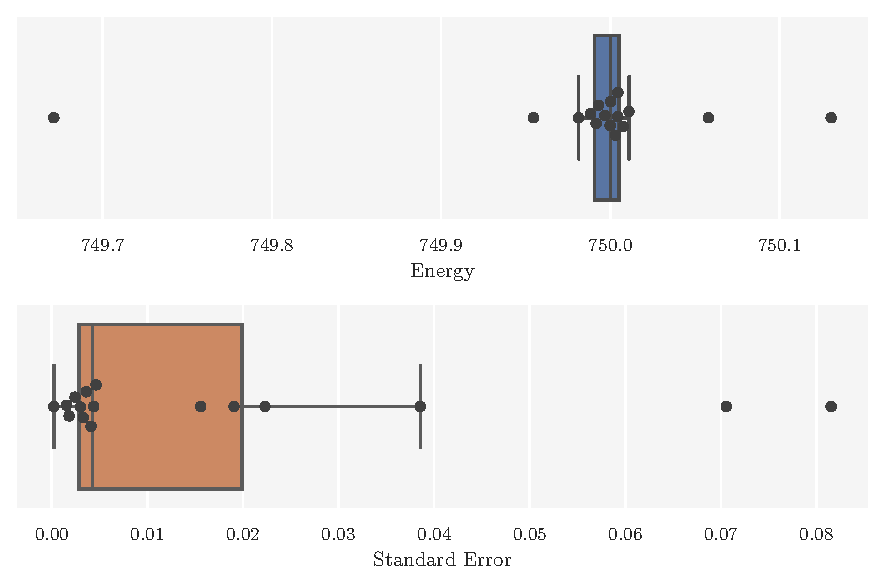
\includegraphics[scale=0.5]{latex/figures/boxplot_numerical_metropolis_hastings.pdf}}}
\caption{\textbf{(a)} Metropolis with analytical. \textbf{(b)} Metropolis-Hastings with analytical. \textbf{(c)} Metropolis with AD. \textbf{(d)} Metropolis-Hastings with AD.}
\label{fig:non-interact_boxplot}
\end{figure}

%----------------------------------------------------------------
\subsubsection{Interacting}
%----------------------------------------------------------------